\section{驱动编写}
为了开发、封装方便,AD9910/AD9854/ADS124S08这几个器件使用同一套模板进行驱动开发,
这套模板是根据Singleton模式设计的,也适用于所有通过串/并口读写寄存器来操作的器件。

下面以ADS124S08为例子进行说明,其他两个器件类似。

\subsection{寄存器定义}
\begin{cbox}{ads124s0x.h}
typedef struct
{
  /* the physical address in the chip */
  const uint8_t addr;
  /* the current value stored locally for transmission */
  uint8_t value;
} ads124s_register;
\end{cbox}

ADS124S08的寄存器都是一个字节长,因此定义较简单。对于AD9854这种不定长的寄存器来说,
还需要一个额外的域来存放长度信息。

\subsection{器件Singleton}
器件相关的所有寄存器都存在一个巨大的结构体单例中。对于ADS124S08,其定义如下:
\begin{cbox}{ads124s0x.h}
typedef struct
{
  ads124s_register id;
  ads124s_register status;
  ads124s_register inpmux;
  ads124s_register pga;
  ads124s_register datarate;
  ads124s_register ref;
  ads124s_register idacmag;
  ads124s_register idacmux;
  ads124s_register vbias;
  ads124s_register sys;
  ads124s_register ofcal0;
  ads124s_register ofcal1;
  ads124s_register ofcal2;
  ads124s_register fscal0;
  ads124s_register fscal1;
  ads124s_register fscal2;
  ads124s_register gpiodat;
  ads124s_register gpiocon;
} ads124s_registers;

/* global struct with shadow registers of the real values which are
 * currently in the ADC */
extern ads124s_registers ads124s_regs;
\end{cbox}

\subsection{寄存器位定义}
\begin{cbox}{ads124s0x.h}
typedef struct
{
  ads124s_register* reg;
  uint8_t bits;
  uint8_t offset;
} ads124s_register_bit;
\end{cbox}

注意在寄存器位\cinl{ads124s_register_bit}的定义中我们嵌入了一个\cinl{ads124s_register}
的指针,这可以在更新配置时帮助我们快速确定其对应的寄存器。

下面是简化寄存器位声明的一个宏:

\begin{minted}{c}
#define DEF_REG_BIT(_name, _reg, _bits, _offset) \
  static const ads124s_register_bit ads124s_##_name = { \
    .reg = &ads124s_regs._reg,  \
    .bits = _bits,              \
    .offset = _offset }
\end{minted}

\begin{figure}[H]
\center
  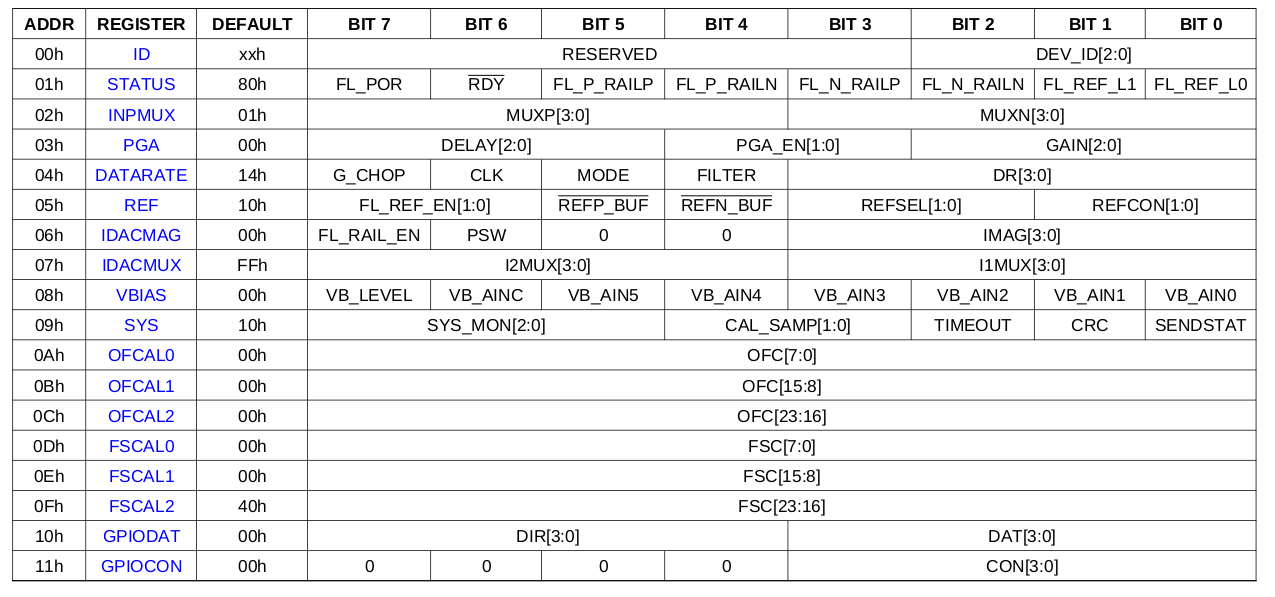
\includegraphics[width=\textwidth]{img/ads124s-regs.png}
  \captionof{figure}{ADS124S0X寄存器图}
\end{figure}

拿PGA这个寄存器来说,如下是定义其3个位域的方法:

\begin{minted}{c}
DEF_REG_BIT(conv_delay, pga, 3, 5);
DEF_REG_BIT(pga_en,     pga, 2, 3);
DEF_REG_BIT(pga_gain,   pga, 3, 0);
\end{minted}

宏展开后会正确定义\cinl{ads124s_conv_delay}、\cinl{ads124s_pga_en}、
\cinl{ads124s_pga_gain}三个静态常量,用于之后的配置。

理论上,还有另一种定义寄存器位的方法,就是使用C语言的位域操作。在设置了按字节对齐的pragma之后,
这样的代码完全能够在ARMv5以上的内核中正确工作,而不必担心访存对齐问题。但是一旦使用位域,
我们就需要为每一个寄存器单独定义一个结构体类型,将会带来很多语法噪音;另一点,
位域的初始化太过麻烦。综合以上,不使用这种语法。

\subsection{常量定义}
为了使用方便,定义器件相关的一些枚举常量:
\begin{cbox}{ads124s0x.h}
typedef enum {
  ads124s_cmd_nop     = 0x00,
  ads124s_cmd_wakeup  = 0x02,
  ads124s_cmd_pwrdwn  = 0x04,
  ads124s_cmd_reset   = 0x06,
  ads124s_cmd_start   = 0x08,
  ads124s_cmd_stop    = 0x0a,
  ads124s_cmd_syocal  = 0x16,
  ads124s_cmd_sygcal  = 0x17,
  ads124s_cmd_sfocal  = 0x19,
  ads124s_cmd_rdata   = 0x12,
  ads124s_cmd_rreg    = 0x20,
  ads124s_cmd_wreg    = 0x40,
} ads124s_cmd_t;
...
\end{cbox}

字面量和类型的前缀尽量和相应的寄存器位保持一致,这样在保证直观的同时也减小出错的概率。
需要注意的是,枚举类型在编译器层面上会被统一为整型,因此尽管它看上去是一个新的类型,
但我们并不能享受到相应的静态类型检查,仅仅是面向代码编写者的一种提示。

\subsection{功能函数}
寄存器位操作的核心函数定义如下:

\begin{cbox}{ads124s0x.h}
static INLINE void
ads124s_set_value(ads124s_register_bit field, uint8_t value)
{
  /* convert the numbers of bits in a mask with matching length */
  const uint8_t mask = ((uint8_t)1 << field.bits) - 1;
  /* clear affected bits */
  field.reg->value &= ~(mask << field.offset);
  /* set affected bits */
  field.reg->value |= ((value & mask) << field.offset);
}

static INLINE uint8_t
ads124s_get_value(ads124s_register_bit field)
{
  /* convert the numbers of bits in a mask with matching length */
  const uint8_t mask = ((uint8_t)1 << field.bits) - 1;
  return (field.reg->value >> field.offset) & mask;
}
\end{cbox}

另一方面,在实现了从器件中读写寄存器的函数后,我们就可以编写更新寄存器的函数了。
有两种方法更新寄存器,一种是直接指出寄存器本身,另一种就是通过寄存器位来间接指代:

\begin{minted}{c}
static INLINE void  /* 直接更新 */
ads124s_update_reg(ads124s_register* reg)
{
  ads124s_write_reg(reg, reg->value);
}

static INLINE void  /* 间接指代 */
ads124s_update_matching_reg(ads124s_register_bit field)
{
  ads124s_update_reg(field.reg);
}

\end{minted}
